%%%%%%%%%%%%%%%%%%%%%%%%%%%%%%%%%%%%%%%%%%%%%%%%%%%%%%%%%%%%%%%%%%%%%%%%%%%%
% AGUtmpl.tex: this template file is for articles formatted with LaTeX2e,
% Modified March 2013
%
% This template includes commands and instructions
% given in the order necessary to produce a final output that will
% satisfy AGU requirements.
%
% PLEASE DO NOT USE YOUR OWN MACROS
% DO NOT USE \newcommand, \renewcommand, or \def.
%
% FOR FIGURES, DO NOT USE \psfrag or \subfigure.
%
%%%%%%%%%%%%%%%%%%%%%%%%%%%%%%%%%%%%%%%%%%%%%%%%%%%%%%%%%%%%%%%%%%%%%%%%%%%%
%
% All questions should be e-mailed to latex@agu.org.
%
%%%%%%%%%%%%%%%%%%%%%%%%%%%%%%%%%%%%%%%%%%%%%%%%%%%%%%%%%%%%%%%%%%%%%%%%%%%%
%
% Step 1: Set the \documentclass
%
% There are two options for article format: two column (default)
% and draft.
%
% PLEASE USE THE DRAFT OPTION TO SUBMIT YOUR PAPERS.
% The draft option produces double spaced output.
%
% Choose the journal abbreviation for the journal you are
% submitting to:

% jgrga JOURNAL OF GEOPHYSICAL RESEARCH
% gbc   GLOBAL BIOCHEMICAL CYCLES
% grl   GEOPHYSICAL RESEARCH LETTERS
% pal   PALEOCEANOGRAPHY
% ras   RADIO SCIENCE
% rog   REVIEWS OF GEOPHYSICS
% tec   TECTONICS
% wrr   WATER RESOURCES RESEARCH
% gc    GEOCHEMISTRY, GEOPHYSICS, GEOSYSTEMS
% sw    SPACE WEATHER
% ms    JAMES
% ef    EARTH'S FUTURE
%
%
%
% (If you are submitting to a journal other than jgrga,
% substitute the initials of the journal for "jgrga" below.)

\documentclass[draft,grl]{AGUTeX}
% To create numbered lines:

% If you don't already have lineno.sty, you can download it from
% http://www.ctan.org/tex-archive/macros/latex/contrib/ednotes/
% (or search the internet for lineno.sty ctan), available at TeX Archive Network (CTAN).
% Take care that you always use the latest version.

% To activate the commands, uncomment \usepackage{lineno}
% and \linenumbers*[1]command, below:

\usepackage{lineno}
\usepackage{amssymb}
\usepackage{amsmath}
\usepackage{textcomp}
\usepackage[super]{nth}
\usepackage{tabularx}
\usepackage{multirow}
\usepackage{bm}
\usepackage{color} 
\usepackage{hyperref}

\linenumbers*[1]

%  To add line numbers to lines with equations:
%  \begin{linenomath*}
%  \begin{equation}
%  \end{equation}
%  \end{linenomath*}
%%%%%%%%%%%%%%%%%%%%%%%%%%%%%%%%%%%%%%%%%%%%%%%%%%%%%%%%%%%%%%%%%%%%%%%%%
% Figures and Tables
%
%
% DO NOT USE \psfrag or \subfigure commands.
%
%  Figures and tables should be placed AT THE END OF THE ARTICLE,
%  after the references.
%
%  Uncomment the following command to include .eps files
%  (comment out this line for draft format):
\usepackage[final]{graphicx}
%
%  Uncomment the following command to allow illustrations to print
%   when using Draft:
%  \setkeys{Gin}{draft=false}
%
% Substitute one of the following for [dvips] above
% if you are using a different driver program and want to
% proof your illustrations on your machine:
%
% [xdvi], [dvipdf], [dvipsone], [dviwindo], [emtex], [dviwin],
% [pctexps],  [pctexwin],  [pctexhp],  [pctex32], [truetex], [tcidvi],
% [oztex], [textures]
%
% See how to enter figures and tables at the end of the article, after
% references.
%
%% ------------------------------------------------------------------------ %%
%
%  ENTER PREAMBLE
%
%% ------------------------------------------------------------------------ %%

% Author names in capital letters:
\authorrunninghead{DAY ET AL.}

% Shorter version of title entered in capital letters:
\titlerunninghead{THE ``SOUTH FLOOD-NORTH DROUGHT'' IN MEIYU AND JET STATS}

%Corresponding author mailing address and e-mail address:
\authoraddr{Corresponding author: Jesse Day, University of California Berkeley, Department of Earth and Planetary Science, College of Letters and Science; 307 McCone Hall, Berkeley, CA 94720, USA. (jessed@berkeley.edu)}

\begin{document}

%% ------------------------------------------------------------------------ %%
%
%  TITLE
%
%% ------------------------------------------------------------------------ %%


\title{Signature of the ``South Flood-North Drought" in Meiyu Front and Tropospheric Jet Changes}

%% ------------------------------------------------------------------------ %%
%
%  AUTHORS AND AFFILIATIONS
%
%% ------------------------------------------------------------------------ %%


%Use \author{\altaffilmark{}} and \altaffiltext{}

% \altaffilmark will produce footnote;
% matching \altaffiltext will appear at bottom of page.

\authors{Jesse A. Day\altaffilmark{1},
Jacob P. Edman\altaffilmark{1}, John C. H. Chiang\altaffilmark{2}, Inez Fung \altaffilmark{1}, and
Weihan Liu\altaffilmark{3}}

\altaffiltext{1}{Department of Earth and Planetary Science, University of California Berkeley, Berkeley, California, USA.}
\altaffiltext{2}{Department of Geography, University of California Berkeley, Berkeley, California, USA.}
\altaffiltext{3}{College of Letters and Science, University of California Berkeley, Berkeley, California, USA.}


%% ------------------------------------------------------------------------ %%
%
%  ABSTRACT
%
%% ------------------------------------------------------------------------ %%

% >> Do NOT include any \begin...\end commands within
% >> the body of the abstract.

%Needs to be 150 words or less - currently at 146.
\begin{abstract}
A novel 57-year (1951-2007) daily catalog of frontal rainbands over China is compiled based on APHRODITE rain gauge data, resulting in an unprecedented climatology of Meiyu front progression in summer. Late \nth{20}-century changes in Chinese summer rainfall are investigated (the ``South Flood-North Drought''). Two robust changes in front behavior are observed during 1980-2007 relative to 1951-1979: 1) A significant decrease in the frequency of frontal rainbands during the Pre-Meiyu period (May), and 2) a southward shift in Post-Meiyu rainbands (mid-July to September). In addition, the mean latitude of the tropospheric jet has shifted southward during both time periods. We propose that the observed changes in frontal rainfall reflect an overall southward displacement of the tropospheric jet's summer progression. By linking East Asian climate change to global change, our results begin to address the critical question of whether the South Flood-North Drought will persist under \nth{21}-century warming.
\end{abstract}

%% Allowed length of manuscript is (# of words/500) + # of figures + # of tables.

%currently: 3509 words + 5 figures (max words: 3500)

\begin{article}

\section{Introduction}
 
 	Eastern China receives about 60\% of its rainfall from May to August via the East Asian summer monsoon. The period of peak rainfall lasting from early June to mid-July is called ``Meiyu season'' (lit. ``plum rains,'' referring to the spectacular growth of plum blossoms in central China with the onset of heavy rains). During this time, heavy rainfall occurs in zonal bands resulting from frontal synoptic conditions (the ``Meiyu front''). The rainfall climatology of Japan and Korea also features similar phenomena known as Baiu and Changma respectively. A growing volume of evidence suggests a shift in rainfall over China beginning in the late 1970s, featuring increased flooding in the south and droughts in the north (the ``South Flood-North Drought'') \citep{Hu1997,Gong2002,Nigam2013}, as shown in Figure \ref{changes_2d}a. Anomalous rainfall patterns have major human impacts on densely-populated eastern China, where many depend on agriculture for subsistence. Northern China suffers from substantial depletion of freshwater resources due to increasing demand \citep{Currell2012,Gleeson2012}. In response, the Chinese government has embarked on a project to reroute water from the Yangtze River to the Yellow River, the South-North Water Transfer Project (\textit{nanshui beidiao gongcheng}), expected to become the most expensive hydraulic engineering project ever undertaken and also entailing massive human and environmental costs \citep{Magee2011}. The severity of the human impacts of the South Flood-North Drought will persist under global warming, or instead represents only a temporary deviation from the long-term mean.
 
	The climatology of the East Asian monsoon bears little resemblance to other monsoon circulations \citep{Ding2005}. Whereas understanding of tropical monsoons has progressed greatly via theoretical studies \citep{Plumb1992,Prive2007,Bordoni2008}, the dynamics that favor the existence of frontal convection over East Asia in summer remain a point of debate, centering around the interplay of the tropospheric jet and Tibetan Plateau \citep{Molnar2010,Sampe2010,Chen2014}. Therefore, no simple conceptual template exists for interpreting a change such as the South Flood-North Drought. However, it is known that the migration of the Meiyu front entails a series of large-scale circulation changes \citep{Chen2004}, and furthermore that anomalies in Meiyu front latitude produce corresponding rainfall anomalies \citep{Kosaka2011}. Therefore, the South Flood-North Drought should be describable in terms of changes in the properties of Meiyu rainbands, such as a shift in latitude, a change in intensity or an earlier or delayed northward migration. In turn, such a characterization may provide insight into the dynamics responsible for the change.
	
	In pursuit of this aim, we have developed a 57-year database (1951-2007) of frontal rainbands in China based on the APHRODITE rain gauge product (described below). We develop a convergent recursive fitting algorithm of daily rainfall maps which determines whether a rainband exists, and if so, quantifies its attributes. Some previous studies have investigated the statistics of the Meiyu front on decadal and even centennial time scales \citep{Chen2004,Ge2008,Xu2009}, but to our knowledge no author has compiled a multi-decadal daily catalog of events. We use this catalog to clarify the spatial and temporal attributes of the South Flood-North Drought, and present it as a tool for future East Asian monsoon research.
		
	We also explore links between the Meiyu front and subtropical jet, which plays an essential and complex role in East Asian climate both in summer and winter \citep{Yang2002}. In a region with strong zonal wind shear such as East Asia, we predict the existence of local meridional circulation producing ascent and frontal rainfall to the south of the core of maximum zonal wind \citep{Holton2004}. Theoretical studies suggest that the high topography of the Tibetan Plateau couples with the jet in nonlinear fashion, amplifying the regional response to global climate anomalies \citep{Nigam1989,Broccoli1992,Park1997}. In summer, past work has argued that the timing of the jet's passage north of the Tibetan Plateau dictates the time of initiation of the Indian and East Asian monsoons, both in present-day \citep{Yin1949,Yeh1959,Hahn1975} and on paleoclimate timescales \citep{Nagashima2011,Nagashima2013,Chiang2015}. Meridional shifts in the tropospheric jet induce rainfall anomalies in China \citep{Liang1998}, as do changes in its strength \citep{Kwon2007,Du2009,Li2014}. On a daily time scale, the jet serves as a waveguide for storms propagating from the Eurasian interior (the ``Silk Road'' teleconnection) \citep{Hoskins1993,Ambrizzi1997,Kosaka2012}. Thus, we expect that changes in the Meiyu front also correspond to \nth{20}-century changes in the East Asian tropospheric jet. Therefore, we compare our rainband database with an existing data set of jet counts for 1958-2001 from \citet{Schiemann2009}, in search of coupled change.
	
\section{Data and Methods}

\subsection{APHRODITE Rainfall Data}

	The APHRO\_MA\_V1101 product from APHRODITE (Asian Precipitation - Highly-Resolved Observational Data Integration Towards Evaluation of the Water Resources) includes 57 years (1951-2007) of daily rainfall (PRECIP product) on a .25\textdegree\ $\times$ .25\textdegree\ grid over Monsoon Asia (60\textdegree E-150\textdegree E and 15\textdegree S-55\textdegree N, units of mm day$^{-1}$) \citep{Yatagai2012}. Values are compiled from rain gauges at weather stations whose daily distribution is indicated by the RSTN product, and are therefore available over land only. We focus on the subregion inside of 100\textdegree E-123\textdegree E and 20\textdegree N-40\textdegree N, where Meiyu rainbands occur. Stations in this region are spaced at 100-200 km intervals, a density sufficient to resolve rainbands. APHRODITE's resolution cannot capture some features visible in TRMM satellite data, such as the anchoring of rainfall in southern China by low coastal orography \citep{Xu2009}. In compensation, the length of APHRODITE data allows the study of decadal change in rainband properties. 
	
\subsection{A Database of Jet Counts from \citet{Schiemann2009}} 

	\citet{Schiemann2009} constructed a data set of jet `counts' in the Tibetan Plateau region (46\textdegree E-130\textdegree E, 17\textdegree N-58\textdegree N) from ERA-40 reanalysis for 1958-2001, where a count is defined as any local maximum in the horizontal wind field with westerly magnitude greater than $30$ m s$^{-1}$; further details can be found in section 2 of \citet{Schiemann2009}. We show daily mean jet latitude averaged across $90-130^\circ$E in Figure \ref{jet_seasonal}a and monthly anomalies in Figure \ref{jet_seasonal}b. Results are not sensitive to the choice of longitude range. Figure \ref{climo} presents contours of jet frequency estimated by a kernel density method, which estimates a probability distribution from a set of discrete data observations (further described in Supplementary Text S3).
	
\subsection{Rainband Detection Algorithm}

	For each day from 1 January 1951 to 31 December 2007 (20,819 days total), a convergent recursive image processing algorithm determines whether a rainband exists inside the window of 105-123\textdegree E and 20-40\textdegree N, defined as a continuous chain of rainfall maxima exceeding 10 mm day$^{-1}$ across more than 5\textdegree of latitude. If one exists, a recursive weighted linear fit is performed of the band's position. Properties of the rainband are calculated including latitude, intensity, tilt, length and width, as well as a ``quality score'' $Q$, defined as the fraction of the day's rainfall that occurred within our fitted band. Days that do not meet a minimum $Q$ value of .6 are excluded. We also test for the possibility of two rainbands occurring on a single day, an arrangement commonly found in August and September. In such a case, the first and second fitted rainbands are referred to as ``primary'' and ``secondary'' respectively. We also discard days dominated by heavy local rainfall over Taiwan. A step-by-step description of the algorithm is presented in Supplementary Text S2 and Supplementary Figures S1-S4, and metrics of its performance documented in Supplementary Tables S1-S3.  It is important to note that our algorithm does not distinguish between the mechanisms that supply rainfall.

\subsection{Bootstrapping and Significance of Changes}

	The standard deviation of rainband frequency and the significance of a change in frequency between two time periods can both be calculated analytically, since frequency follows a Bernoulli distribution. However, it cannot be assumed that front and jet data are normally distributed. Instead, we use bootstrapping with replacement to calculate the standard deviation of daily mean jet latitude and rainband properties (Figure \ref{jet_seasonal}a and Supplementary Tables S4-S8 respectively). To calculate the statistical significance of the difference in means between samples, two methods are used: 1) Bootstrapping with replacement and 2) a permutation test (bootstrapping without replacement) \citep{Good2005}. By drawing new samples from actual data and taking their mean for 10,000 iterations, we obtain a synthetic distribution of differences, and compare the actual difference to this distribution to estimate a $p$-value. In the rest of the text we show the results of permutation testing, which produces results very similar to those obtained by bootstrapping with replacement, but generally stricter ($p$-value closer to .5). We focus on changes in front attributes between 1951-1979 and 1980-2007 (Supplementary Tables S5 and S6). We also successfully verified that these results are robust to using only years where jet data is available (1980-2001 versus 1958-1979; not shown).
	
\section{Rainband Statistics}	
	
\subsection{Climatology}	

	The yearly progression of precipitation over eastern China is shown in Figure \ref{hov}a, longitudinally averaged over $100-123^\circ$E with a 5-day running mean, similar to Figure 7 in \citet{Ding2005}. China receives a substantial fraction of its yearly precipitation outside of summer, unlike other monsoonal regions \citep{Wang2002}. Figure \ref{hov}b shows a Hovm\"oller diagram of the frequency of rainbands over all 57 years, including both primary and secondary rainbands. Some periods of heavy rainfall, in particular the August peak over southern China (over 10 mm day$^{-1}$ around 20\textdegree N), do not correspond to a surge in rainbands. Figure \ref{hov}c shows the probability of observing a rainband and mean rainband intensity, and Figure \ref{hov}d shows mean rainband tilt and length, as well as the conditional probability of observing a secondary rainband given the presence of a primary rainband. Frontal rainbands over China can appear in any month, with their probability of occurrence and intensity maximizing in late June (80\% probability of occurrence, mean intensity of 31 mm day$^{-1}$) and minimizing in January (10\% probability occurrence, mean intensity of 12 mm day$^{-1}$).
	
	Coordinated sharp changes occur in rainfall and frontal properties. We define 5 periods of notable frontal behavior as demarcated in Figure \ref{hov}: 1) The ``Spring Rains'' (days 60-120, March 1-April 30), as previously studied in \citet{Tian1998}; 2) The ``Pre-Meiyu'' (121-160, May 1-June 9), during which rainfall and front intensity increase; 3) Meiyu season (161-200, June 10-July 19) when a remarkable 7-degree northward shift in mean rainband latitude occurs over the course of several weeks, and rainband frequency and intensity peaks; 4) The Post-Meiyu (201-273, July 20-September 30), during which double rainbands are common; and 5) the ``Fall Rains'' (274-320, October 1-November 16), when rainband latitude returns south. The Pre-Meiyu, Meiyu and Post-Meiyu are equivalent to the three stages of Meiyu rainfall described in \citet{Ding2005}. Our results can also  be compared with the event catalog of \citet{Xu2009}, which finds a similar date for the northward transition of the Meiyu front. The total number of rainband counts and mean and standard deviation of rainband frequency, latitude and intensity during each time period are presented in Supplementary Table S4.  In addition, Figures \ref{climo}a-e show mean rainfall, jet frequency and rainband position during each of these stages, as well as their zonal average (sidebars). From the Pre-Meiyu to Post-Meiyu, the northward progress of peak rainband frequency corresponds to a similar shift in jet count density, with a southward offset of about 5 degrees. A yearly asymmetry can also be seen between more frequent and intense rainbands during the jet's northward passage (Pre-Meiyu and Meiyu) versus weaker rainfall during its southward return (Fall Rains), which merits further study.
		
\subsection{Changes in Rainband Attributes, 1980-2007 Versus 1951-1979}
	
	We calculate changes in rainfall (Figure \ref{changes}a) and rainband frequency, latitude and intensity (Figure \ref{changes} and Supplementary Tables S5 and S6) during 1980-2007 versus 1951-1979, as well as the changes' statistical significance. In addition, Figures \ref{changes_2d}b and \ref{changes_2d}c show spatial changes in rainfall and jet count density during the Pre-Meiyu and Post-Meiyu, when changes are particularly large. During the Pre-Meiyu (days 121-160), the probability of observing a primary rainband has declined sharply from $59.0\% \pm 1.4\%$ to $53.0\% \pm 1.5\%$ (statistical significance of $p=0.0019$; Table S5). A corresponding decrease in Pre-Meiyu rainfall has occurred in central China (Figure \ref{changes_2d}b and 30\textdegree N in Figure \ref{changes}a). The change in Pre-Meiyu rainfall in the late \nth{20} century has previously been reported by \citet{Xin2006} and \citet{Wang2009}.
		
	In addition, a southward shift in mean rainband latitude has occurred during the Post-Meiyu (days 201-273, or July 20-Sep 30). Considering both primary and secondary rainbands north of 27\textdegree N, which are associated with the jet (Figure \ref{climo}d and Figure \ref{jet}c), mean latitude during 1951-1979 was $33.6^\circ \textrm{N} \pm .3^\circ$ versus $32.9^\circ \textrm{N} \pm .3^\circ$ during 1980-2007 (statistical significance $p=.0003$; Table S6). This shift remains significant if we do not restrict by front latitude ($p=.0048$). A Post-Meiyu rainfall increase in central China and decrease in northern China has occurred, producing a South Flood-North Drought pattern (Figure \ref{changes_2d}c). As a result, yearly rainfall has increased in central China even though Pre-Meiyu rainfall changes in that region are negative (Figure \ref{changes_2d}a). Unlike \citet{Yu2010}, our catalog does not exhibit a \nth{20}-century decrease in the intensity of Yangtze River region frontal rainbands during July-August. A significant southward shift in rainband latitude is also found for the whole year ($p=.0032$, Table S6), but this signal is dominated by the Post-Meiyu shift.
	
\section{Jet}

\subsection{Dynamics}

	The tropospheric jet marks the northern boundary of the Hadley Cell, and shifts in response to seasonal changes in insolation \citep{Bordoni2008}. Beginning in May, the East Asian jet shifts from its winter position on the southern flank of the Tibetan Plateau to a summer latitude well north of the plateau. During this transition, the jet occupies intermediate configurations that correspond to different stages of China rainfall (Figure \ref{climo}). A full monthly jet climatology is visible in \citet{Schiemann2009}. Peak rainfall rates in China from May to mid-July corresponds to the months when the climatological latitude of the jet impinges on the Tibetan Plateau. The interaction of the tropospheric jet and Tibetan Plateau strengthens convergence and rainfall downstream over China and the western Pacific Ocean \citep{Molnar2010,Sampe2010,Chen2014}. From May to September,  the climatological latitude of rainfall, rainbands and jet density are all closely coupled, with peak jet density occurring 5 to 10 degrees north of the latitude of peak rainfall. The initiation of the Pre-Meiyu corresponds roughly to the beginning of the jet's northward passage. During Meiyu season, the preferred latitude of the jet continues to shift northward. The period of frequent double rainband occurrence during the Post-Meiyu corresponds to the jet's maximal northward extent. Finally, the Fall Rains in October and November correspond to the southward return of the jet, which produces only a weak rainfall response.
	
\subsection{Jet Changes, 1980-2001 Versus 1958-1979}

	In Figure \ref{jet_seasonal}a, we show the zonal average over $90-130^\circ$E) of mean jet latitude, averaged over the years 1958-1979 (blue solid line) and 1980-2001 (dashed red line) with 95\% confidence intervals overlain. Both significant changes in rainband statistics described in the previous section correspond to southward shifts in mean jet latitude. During the Pre-Meiyu (May), the tropospheric jet is shifted southward by almost 2\textdegree\ in 1980-2001 relative to 1958-1979, when its mean latitude was $\approx 41^\circ$N. We estimate the significance of this change using a two-tailed Kolmogorov-Smirnov (K-S) test. Since the K-S test requires that all samples are independent, we first remove temporal autocorrelation due to synoptic variability by assimilating daily mean jet latitude into 4 day blocks (Supplementary Figure S5). A subsequent K-S test finds that the shift is significant with $p=0.003998$. During the Post-Meiyu (days 201-273), when a southward shift in rainband latitude was found in 1980-2001 relative to 1958-1979, the mean latitude of the jet is also consistently displaced southward. We assimilate daily mean jet latitude into 7-day blocks (Supplementary Figure S5) before performing a K-S test, and find a $p$-value of the jet shift of $p=0.05667$.
		
\section{Discussion}

	The Meiyu front and tropospheric jet covary in latitude from May to September in the climatological mean, and parallel changes are found in rainband attributes and mean jet latitude between 1951-1979 and 1980-2007. Therefore, the South Flood-North Drought appears to reflect an alteration in jet dynamics. We propose that both the Pre-Meiyu decline in rainband frequency and the Post-Meiyu southward shift of rainband latitude result from a single phenomenon: an overall southward displacement of the jet's summer progression over East Asia. In climatology, the Pre-Meiyu corresponds to both a surge in rainfall and the beginning of the jet's northward transit, when its preferred latitude begins to impinge on the Tibetan Plateau. We propose that the observed southward shift in the jet during May has delayed the date when the jet first impinges on the Tibetan Plateau, resulting in a delay in Pre-Meiyu onset and prolonged Spring Rain conditions. This is manifested as weaker rainfall and decreased rainband frequency in central China in May. Subsequently, we argue that the reduced northward extent of the jet during the Post-Meiyu has shifted rainfall and mean rainband latitude southward. Finally, we suggest that the southward displacement of the summer jet cycle results in a decrease in northern China annual rainfall and an increase in central China annual rainfall, producing a South Flood-North Drought response. Thus, our hypothesis can explain the major observed changes in rainfall and rainband statistics during the Pre- and Post-Meiyu as well as cumulative yearly change.
	
	To test our hypothesis, we investigate the relation of interannual anomalies in jet latitude and rainband properties. Figure \ref{jet_seasonal}b shows a scatter plot of rainband \textit{frequency} anomalies versus jet latitude anomalies in May (days 121-150). Most years with a decrease in rainband frequency feature a southward jet shift, and vice-versa, and such years occur mostly during 1980-2007. A similar relation is found between monthly anomalies in rainband \textit{latitude} and jet latitude during July-August (days 201-260, Figure \ref{jet_seasonal}c). In the latter figure, we exclude rainbands south of 28\textdegree N from calculated anomalies, since such rainbands reflect South China Sea storms, rather than jet influence \citep{Day2015}. Together, Figures \ref{jet_seasonal}b and \ref{jet_seasonal}c suggest that interannual changes in jet latitude alter Pre-Meiyu rainband frequency and Post-Meiyu rainband latitude.

	 Observations show that the global annual mean latitude of the tropospheric jet has shifted poleward, in tandem with tropospheric heating and lower-stratospheric cooling in the mid-latitudes, increased subtropical static stability, and the expansion of the Hadley circulation \citep{Fu2006,Archer2008,Fu2011}. Opposite trends are found in some regions and the variation by season is significant; we find that the East Asian portion of the jet has shifted equatorward, in agreement with past studies \citep{Yu2007, Archer2008}. Recent work suggests that the southward displacement of the jet over the Pacific Ocean was caused by \nth{20}-century changes in tropical Pacific convection and SST \citep{Park2014a}. Thus, the global poleward trend in jet latitude and the East Asian equatorward shift are compatible observations that reflect the heterogeneous spatial distribution of \nth{20}-century warming.
	 
	 In addition to the late 1970s change in China rainfall, earlier onset of rainfall over the South China Sea during 1994-2008 relative to 1979-1993 has been reported \citep{Kajikawa2012}, as well as an increase in rainfall over southern China and in the passage of tropical cyclones \citep{Kwon2007,Chang2014}. In Supplementary Tables S7 and S8, we find a rise in rainband intensity during Meiyu season (days 161-200) from 27.3 to 29.8 mm day$^{-1}$ ($p=.9994$), and a southward shift in rainband latitude from 30.0\textdegree N to 28.9\textdegree\ N ($p=.0002$). No significant changes are found in rainband frequency or jet latitude. The strengthening and southward shift of Meiyu season rainbands beginning in the mid-1990s merits further investigation.
		
\section{Conclusion}

	We have shown that a significant amount of the annual and decadal variability in Meiyu front activity is accompanied by changes in the westerly jet. Using a recursive convergent image processing algorithm, we created an unprecedented database and 57-year climatology of frontal rainfall properties over China, including probability of rainband occurrence and mean latitude, intensity, tilt, width and length. Two statistically significant changes in rainband attributes occurred between the years 1951-1979 and 1980-2007: 1) A decrease in frequency during the Pre-Meiyu season (days 121-160, May 1-June 9; $p=.0019$); and 2) A southward shift in rainband latitude during the Post-Meiyu season (days 201-273, July 20-Sep 30; $p=.0003$). The latter change is responsible for the South Flood-North Drought trend in total yearly rainfall. In addition, both time periods display a southward anomaly in mean jet latitude during 1980-2007 relative to 1951-1979. We argue that both Pre-Meiyu and Post-Meiyu changes in rainfall and rainband statistics are caused by a southward shift of the summer progression of the East Asian tropospheric jet. In particular, we propose that the delayed passage of the jet to the north of the Tibetan Plateau has shortened the Pre-Meiyu season, decreasing May rainfall in central China, and restricted the northward advance of precipitation, consequently reducing Post-Meiyu rainfall in northern China. This interpretation is a modern analog of the ``Jet Transition Hypothesis'' described in \citet{Chiang2015}, wherein East Asian rainfall changes on paleoclimate time scales are ascribed to modulation in the seasonal cycle of the tropospheric jet. 	
 
	Many components of our results have been presented in previous work. \citet{Xuan2011} find a southward shift in the jet and increased Yangtze Valley rainfall in July. \citet{Yu2004} and \citet{Yu2007} found a southward shift in July-August jet latitude and suggested a link with the South Flood-North Drought. Potential mechanisms for late \nth{20}-century East Asian climate change include changes in Indian Ocean SST \citep{Qu2012}, decreased sensible heating from the Tibetan Plateau \citep{Liu2012a,Hu2015} and aerosol forcing \citep{Song2014}. Other studies attribute the South Flood-North Drought to natural variability \citep{Zhang1999,Xin2006,Lei2014}, but \citet{Zhou2009} claimed that the South Flood-North Drought was distinct from other patterns of \nth{20}-century variability. Our hypothesis, that the altered seasonal cycle of the jet induces observed rainfall change, does not supplant prior explanations but rather provides further observations that they must address.
	 
	It is essential to understand whether the South Flood-North Drought will persist under \nth{21}-century warming, or manifests an ephemeral decadal change. However, the CMIP5 (Climate Model Intercomparison Project) model suite contained in the Intergovernmental Panel on Climate Change's Fifth Assessment Report (IPCC AR5) does not agree on the sign of future summer rainfall changes in East Asia \citep{Christensen2011}. In this study, we have tied the regional rainfall climate of China to the seasonal progression of the westerly jet, which is a larger-scale feature and therefore more easily studied in global climate models and idealized studies. The poleward expansion of the Hadley Cell is projected to continue under \nth{21}-century warming \citep{Lu2007,Kang2012}, but a recent study predicts that anomalous \nth{21}-century heating of the eastern Pacific Ocean will drive the Pacific jet further equatorward \citep{Park2014}. By linking the South Flood-North Drought to changes in the seasonal advance of the tropospheric jet, we open the possibility of projecting \nth{21}-century East Asian rainfall change by improving our understanding of the effect of further global warming on the regional and global behavior of the tropospheric jet.
	

%%%  ACKNOWLEDGMENTS

\begin{acknowledgments}
This work was supported by NSF grants AGS-1405479, EAR-0909195 and EAR-1211925, which allowed the presentation of preliminary results in conference settings and the feedback of our peers. We also acknowledge NSFC (National Natural Science Foundation of China) grant \#40921120406 for enabling our collaboration with Professor Yanjun Cai of IEECAS in Xi'an, which led to the present work. We thank Reinhardt Schiemann for sharing his database of jet counts. APHRODITE precipitation data is publicly available at \url{http://www.chikyu.ac.jp/precip/index.html}. FERRET, a NOAA product, was used for data analysis and preliminary plot generation. We also thank Gerard Roe for a valuable comment on the poleward global shift of jet latitude. A full database of rainband statistics from 1 January 1951 to 31 December 2007 is available upon request.
\end{acknowledgments}

\bibliographystyle{agufull08}
\bibliography{meiyu}

%% ------------------------------------------------------------------------ %%
%
%  END ARTICLE
%
%% ------------------------------------------------------------------------ %%
\end{article}
%
%
%% Enter Figures and Tables here:
%
% DO NOT USE \psfrag or \subfigure commands.
%
% Figure captions go below the figure.
% Table titles go above tables; all other caption information
%  should be placed in footnotes below the table.
%


%%% Hovm�ller diagram of Meiyu latitude occupancy, 1951-2007. Produced by MATLAB scripts meiyufig1.m and meiyustats_compact.m.
\begin{figure}
\label{hov}
\noindent\includegraphics[width=36pc]{Figures/meiyu_hovmoller}
\caption{Hovm\"oller climatology of East Asian rainfall, 1951-2007, with important time periods marked as follows: 1 - Spring Rains; 2 - Pre-Meiyu; 3 - Meiyu; 4 - Post-Meiyu; 5 - Fall Rains. a) Precipitation averaged over the longitudes 100-123\textdegree E. b) Probability of occurrence of a rainband for each day and latitude (both primary and secondary, in percentage), smoothed in time with a 9-day running box filter c) Probability of primary rainband occurrence and mean intensity (9-day running mean) d) The conditional probability of a secondary rainband given the presence of a primary rainband, as well as the mean tilt and length of primary rainband events (9-day running mean).}
\end{figure}

%Climatology of rainfall stages including rainfall, jet and most likely rainband configuration, and longitudinal averages.
\begin{figure}
\label{climo}
\noindent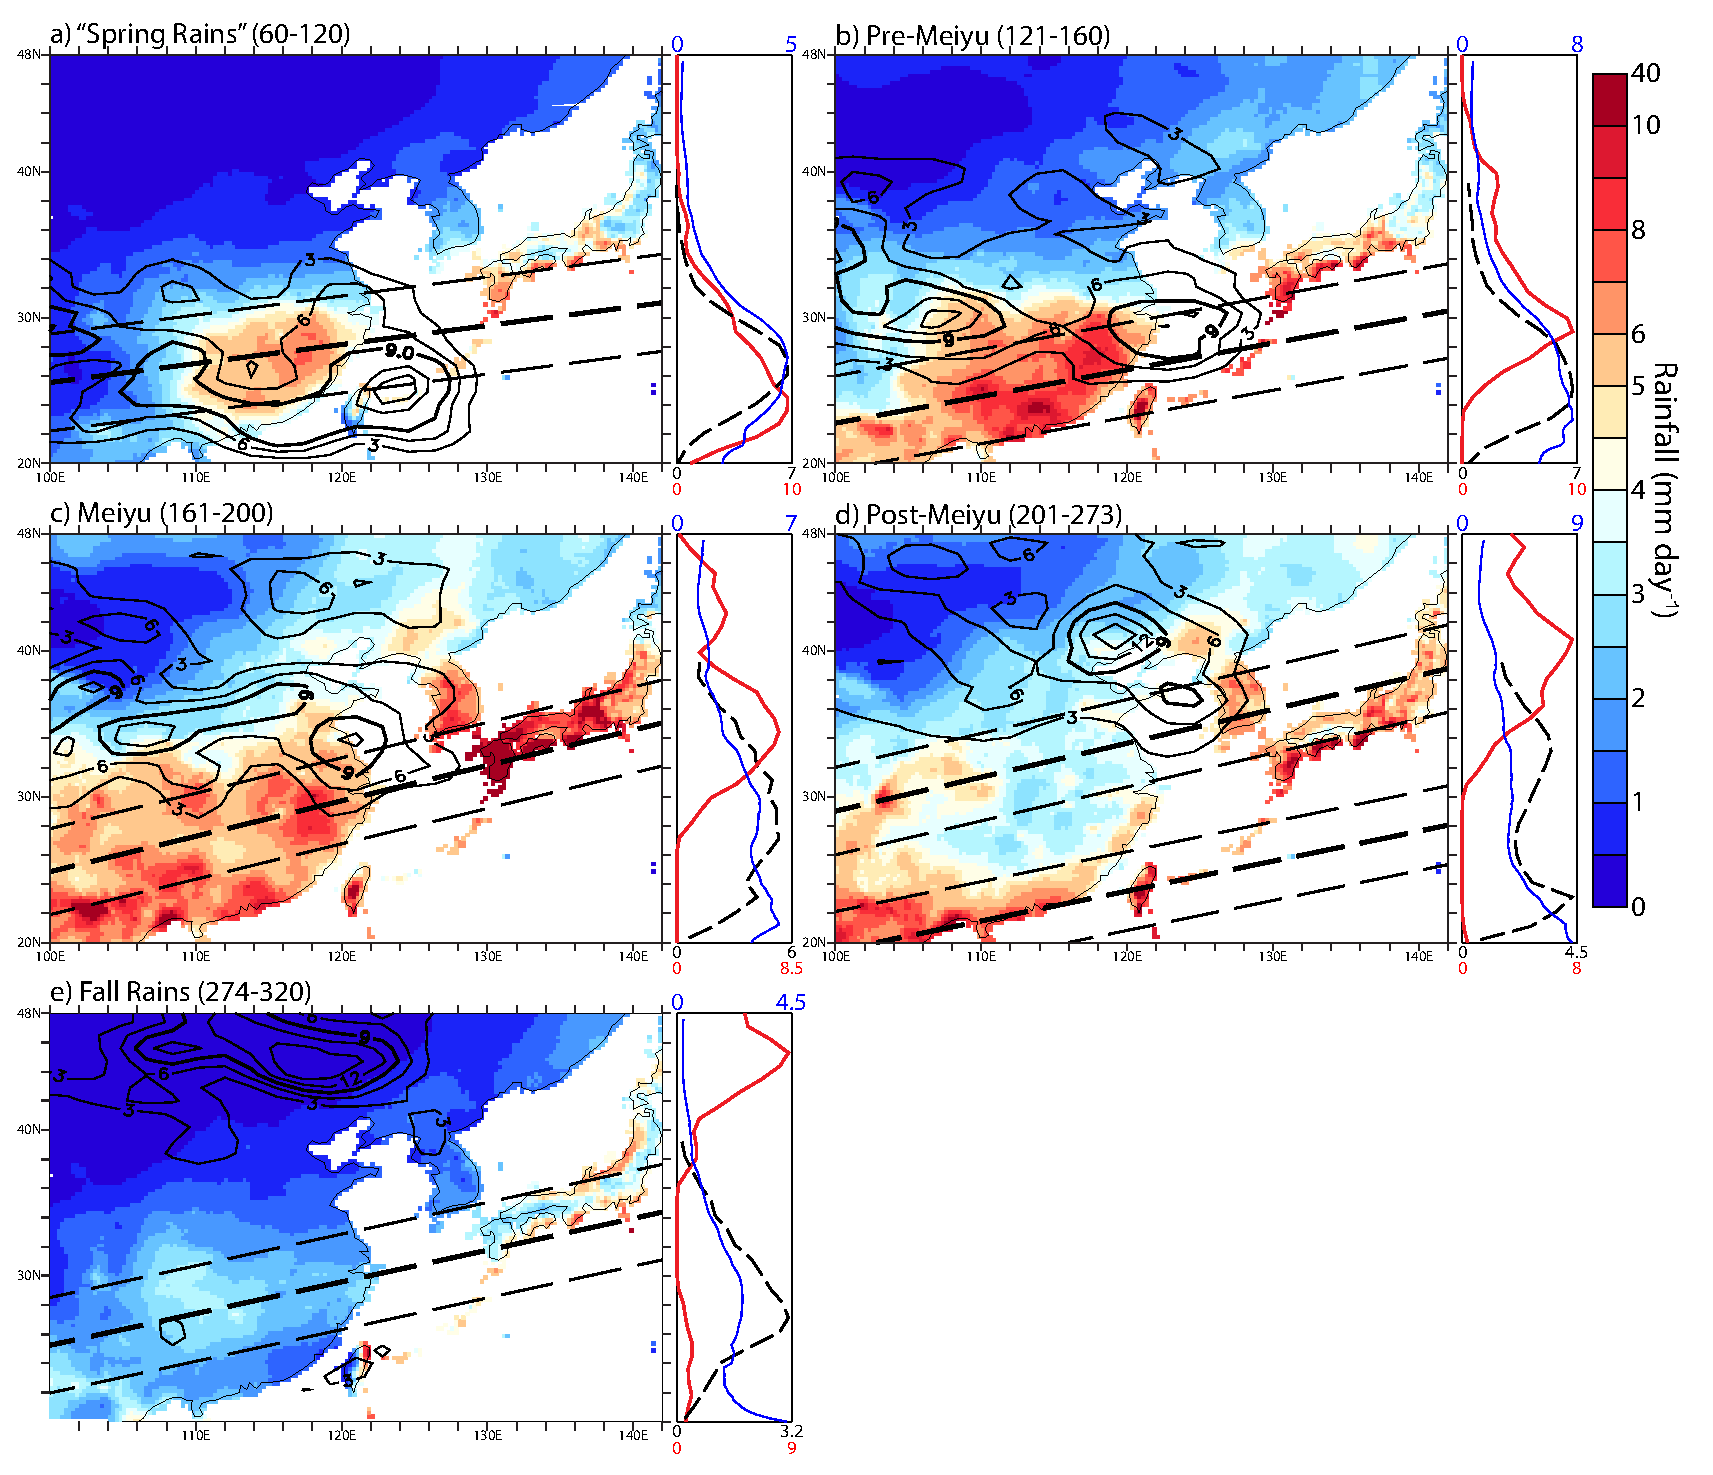
\includegraphics[width=36pc]{Figures/climo}
\caption{Climatology of East Asian rainfall stages showing rainfall (colors), jet kernel density (contours of probability density in units of $10^{-4}$) and most common rainband position during that stage. Sidebar on the right of each figure shows, for the given time period, the longitude average over 105-123$^{\circ}$E of rainfall (thin blue line, units of mm day$^{-1}$) and jet kernel density (dashed black line, units of $10^{-4}$) as well as rainband position (thick red line, absolute probability in \%, 9-day running mean and 1-degree latitude smoothing). From the Pre-Meiyu to Post-Meiyu, a peak in preferred jet latitude consistently occurs 5 degrees north of a corresponding maximum in rainband frequency.}
\end{figure}

%%% Changes in Meiyu and rainfall behavior between 1951-1979 and 1980-2007
\begin{figure}[htbp]
\begin{center}
\includegraphics[width=36pc]{Figures/changes}
\caption{a) 15-day running mean of the change in rainfall between 1951-1979 and 1980-07, with 95\%/99\% confidence level marked by single/double cross-hatches. b) 15-day running mean of the change in rainband frequency between 1951-1979 and 1980-07, with two-degree smoothing in latitude and confidence levels marked as in a). In both cases, significance is calculated by bootstrapping over a 15-day running window; for Meiyu frequency, a two-degree latitude window is also used (see Appendix for further description). Time periods are marked as in Figure 1.}
\label{changes}
\end{center}
\end{figure}

%2D spatial distribution of change showing a) full year b) Pre-Meiyu and c) Post-Meiyu
\begin{figure}
\noindent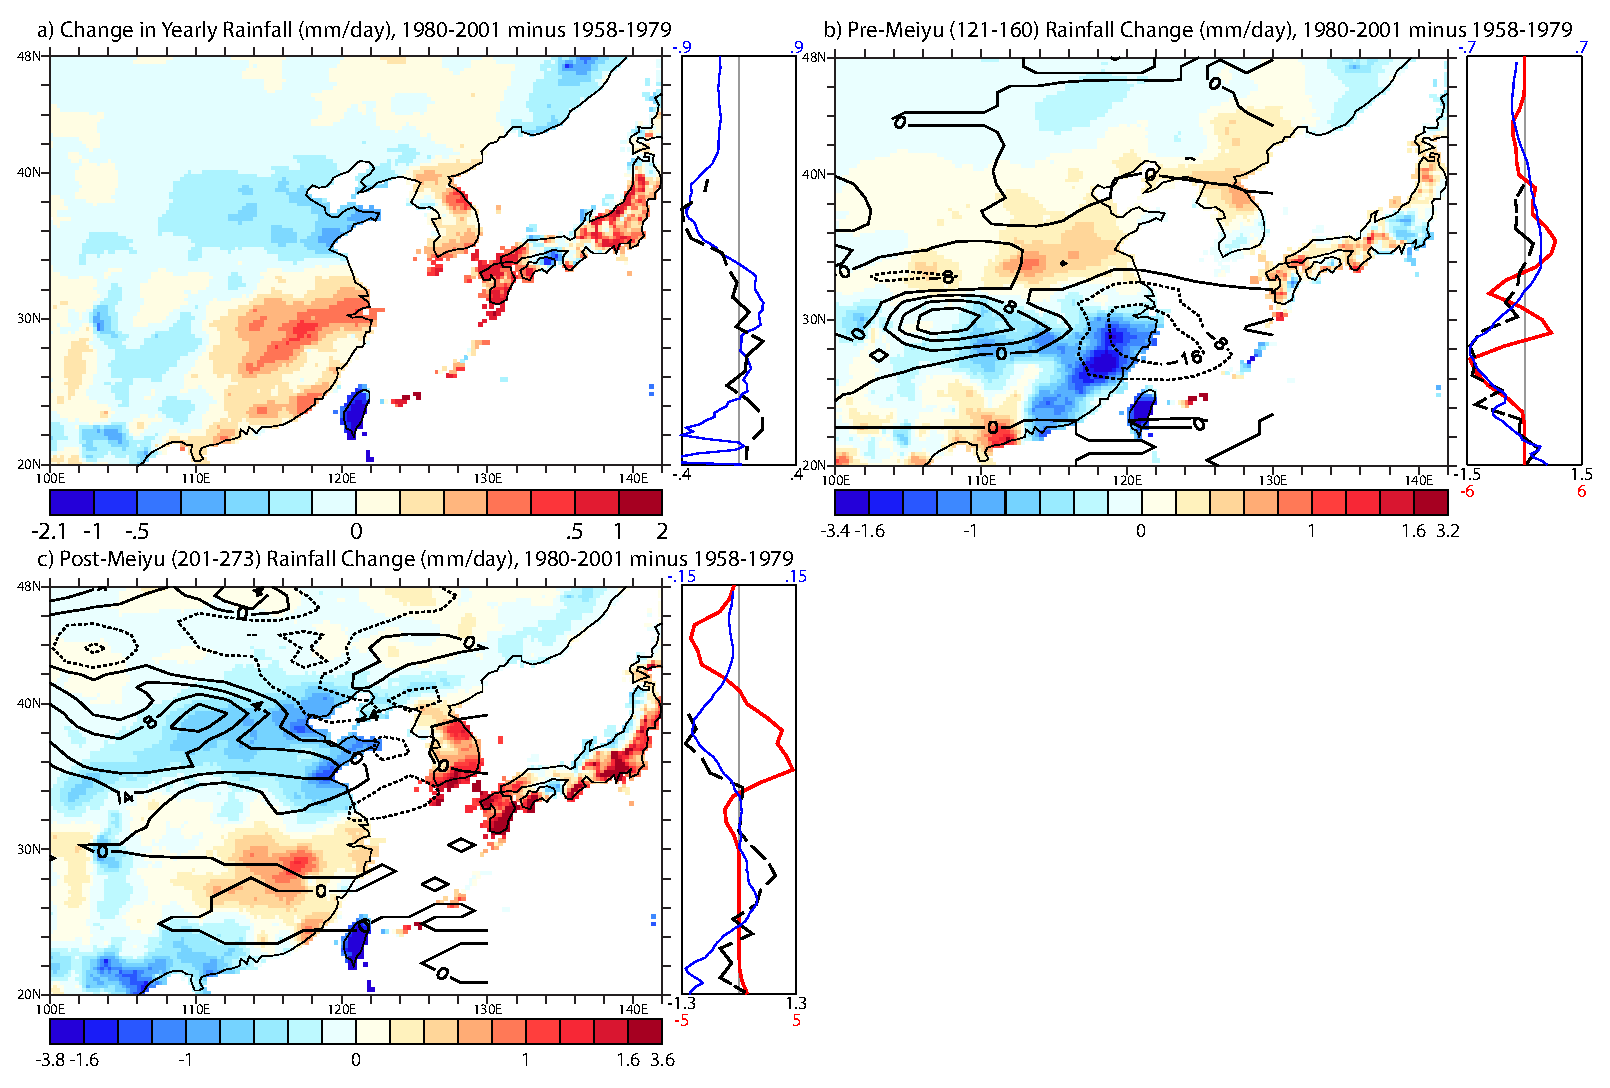
\includegraphics[width=36pc]{Figures/changes_2d}
\caption{a) The South Flood-North Drought pattern of all-year rainfall change; b) Rainfall changes during the Pre-Meiyu (days 121-160) with contours of jet density change overlain; c) Same as c, but for the Post-Meiyu (days 201-273). Sidebar on the right of each figure shows, for the given time period, the longitude average over 105-123$^{\circ}$E of changes in rainfall (thin blue line, units of mm day$^{-1}$) and jet kernel density (dashed black line, units of $10^{-4}$) as well as rainband position (thick red line, absolute probability in \%).}
\label{changes_2d}
\end{figure}

%%% Changes in jet mean between 1951-1979 and 1980-2007 + scatter plots of jet and rainband monthly anomalies.
\begin{figure}[htbp]
\begin{center}
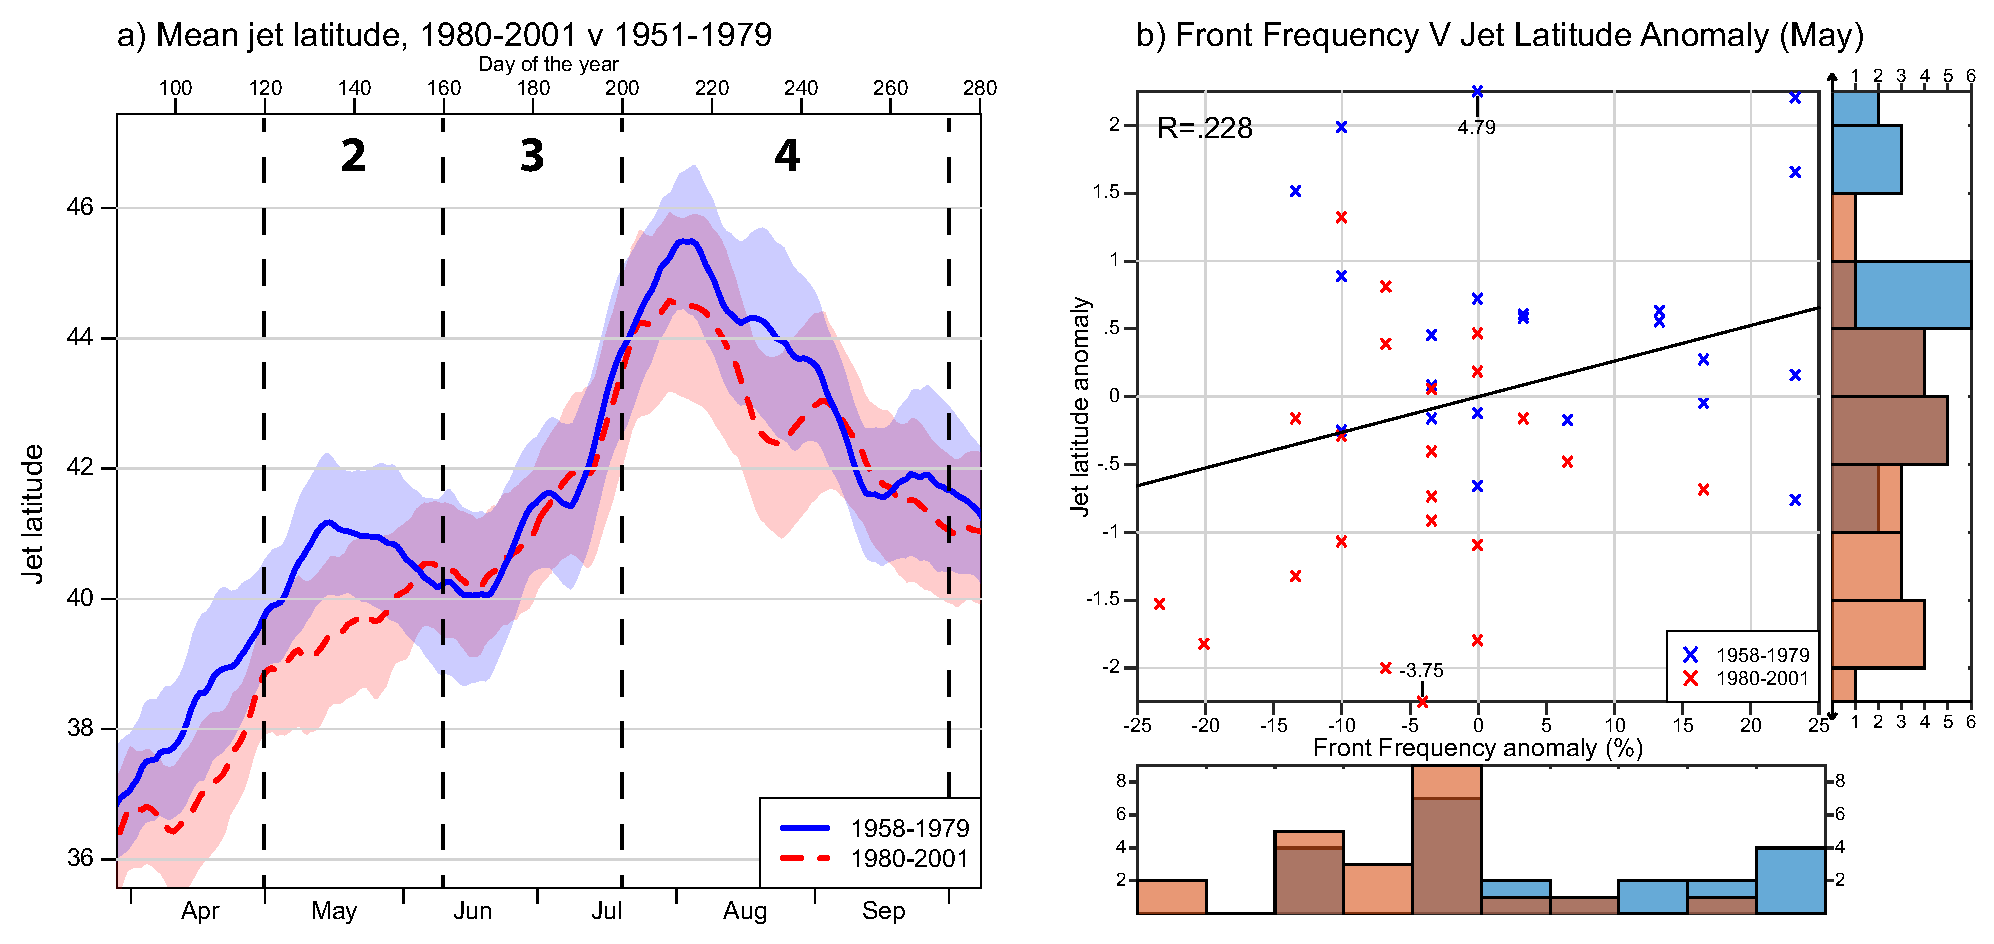
\includegraphics[width=42pc]{Figures/jet}
\caption{a) 7-day running mean latitude of the westerly jet in the region 90-130$^\circ$E for the 1958-1979 (blue, solid) and 1980-2001 (red, dashed). Bootstrapped 95\% confidence intervals are shaded. Time periods: 2 - Pre-Meiyu; 3 - Meiyu; 4 - Post-Meiyu; b) Plot of monthly anomalies in rainband frequency versus monthly anomalies in jet latitude during days 121-150 (May) for 1958-1979 (blue) versus 1980-2001 (red), with anomalies also shown in histogram form.}
\label{jet_seasonal}
\end{center}
\end{figure}

\end{document}